%!TEX root = ../my_thesis.tex
\chapter{Architecture matérielle de correction des erreurs résiduelles}

Texte Intro

- Etat de l'art des archi mat de tdec pour voir comment interfaecer une architecture matérielle de l'algorithme FNC avec
des turbo décodeurs de la littérature.
- Etude des impacts des paramètres
- Cas d'étude : Architecture matérielle adaptée à un turbo décodeur seq FB-SW
- Projections sur l'extension à d'autres ordonnancements de tdec
- cl
\vspace*{\fill}
\minitocTITI
\vspace*{\fill}
\newpage

\section{Les architectures matérielles de turbo décodeurs}
Dans cette section, un état de l'art des architectures de turbo décodeurs est mené. Dans un premier temps, des détails 
sont donnés pour des architectures basées sur un processus itératif de turbo décodage séquentiel. Des architectures 
matérielles réalisant plusieurs demi-itérations en parallèle seront présentées dans un second temps.

\subsection{Processus itératif séquentiel}
Le décodage des turbo codes est basé sur l'échange d'informations extrinsèques entre différents décodeurs SISO. À partir 
des informations du canal et des informations \textit{a priori}, chaque décodeur SISO évalue les informations 
\textit{a posteriori}. De là, en sont déduites les informations extrinsèques qui sont alors utilisées en tant
qu'informations \textit{a priori} lors de la demi-itération suivante conjointement avec les informations de l'autre
domaine. La Figure \ref{fig:turbo_seq} présente la séquentialité de ces opérations lors du processus de décodage
itératif. Il apparaît qu'un seul décodeur SISO est implémenté. 
%Au cours des itérations, cet unique décodeur 

\begin{figure}[!h]
	\centering
	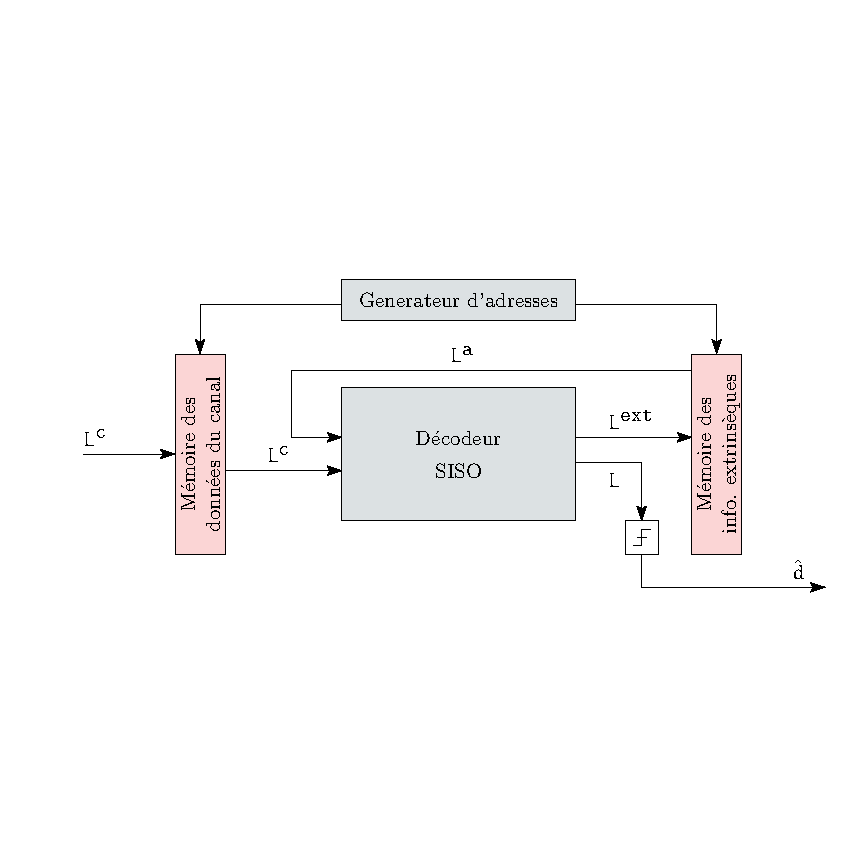
\includegraphics{main/ch4_fig/ipe/serial.pdf}
	\caption{Turbo décodage séquentiel. \label{fig:turbo_seq}}
\end{figure} 

L'algorithme de décodage SISO choisi permettant l’obtention des informations \textit{a posteriori} est l'algorithme MAP, 
ou plutôt une des ses simplifications comme l'algorithme EML-MAP. Cet algorithme repose sur trois calculs successifs et 
séquentiels. Suivant l'ordonnancement choisi et le degré de parallélisme choisi pour ces calculs, différentes valeurs 
de besoins en ressources calculatoire ou de mémorisation, de temps d'exécutions peuvent être obtenus. Un détail, 
incrémental de ces différentes approches est maintenant mené, suivant la classification proposée par \cite{Muller2010}.

\subsubsection{BCJR séquentiel}
\paragraph*{BCJR aller-retour}
Les étapes de l'algorithme BCJR sont détaillés ci-après. Tous d'abord, le calcul des métriques de branches, notées 
$\gamma$, est réalisé. Ceci permet d’entamer le calcul récursif des métriques de nœuds aller, notées $\alpha$. Chaque 
métrique de nœud aller est calculée en combinant la transition du treillis courante avec les métriques $\alpha$ de la section de treillis précédente. Le calcul récursif des métriques de nœuds retour, notées $\beta$, est similaire mais
considère un parcours du treillis du code dans l'autre sens, en partant de la fin du treillis. Finalement, les 
informations \textit{a posteriori} sont calculées en combinant ces trois métriques $\alpha$, $\beta$ et $\gamma$. 

Comme dans le cas de l'algorithme de Viterbi, chaque calcul de métrique de nœud est réalisé par un opération ACS 
(Addition-Comparaison-Sélection). En multipliant le nombre d'unités ACS par le nombre de nœuds d'une section du treillis 
du code, il est possible de calculer toutes les métriques de nœud (aller ou retour) d'une même section en même temps. Ce
parallélisme ne nécessite que peu de surcoût matériel puisque seulement les unités ACS sont dupliquées sans nécessiter
de mémorisation supplémentaire car chaque opération d'ACS est exécutée sur le même jeu de données. Ainsi, l'ensemble des
métriques de nœud d'une section de treillis peut être calculé en un coup d'horloge. Le calcul récursif des métriques de 
nœuds nécessite alors K cycles d'horloge.

L'instant suivant le calcul de la métrique de nœud retour, il est possible d'effectuer le calcul de l'information 
\textit{a posteriori}. C'est ordonnancement des opérations correspond à celui originellement proposé par Bahl, Cocke, Jelinek et Raviv lors de la présentation de leur algorithme de décodage \cite{bcjr}. Dans le suite de ce manuscrit, cet
ordonnancement des opérations est nommé Forward-Backward (FB). Il est schématisé dans la Figure \ref{fig:siso_seq}.
Il apparaît que sans considérer les bits de terminaison du treillis -- qui ne sont jamais pris en compte dans ce chapitre afin d'exprimer plus simplement les nombre de cycles nécessaire -- le temps requis pour exécuter une demi-itération du processus de décodage itératif équivaut à $2\times K$ cycles d'horloge. Il est nécessaire de mémoriser
les K métriques de nœuds aller afin de pouvoir obtenir les informations \textit{a posteriori}.

\begin{figure}[!h]
	\centering
	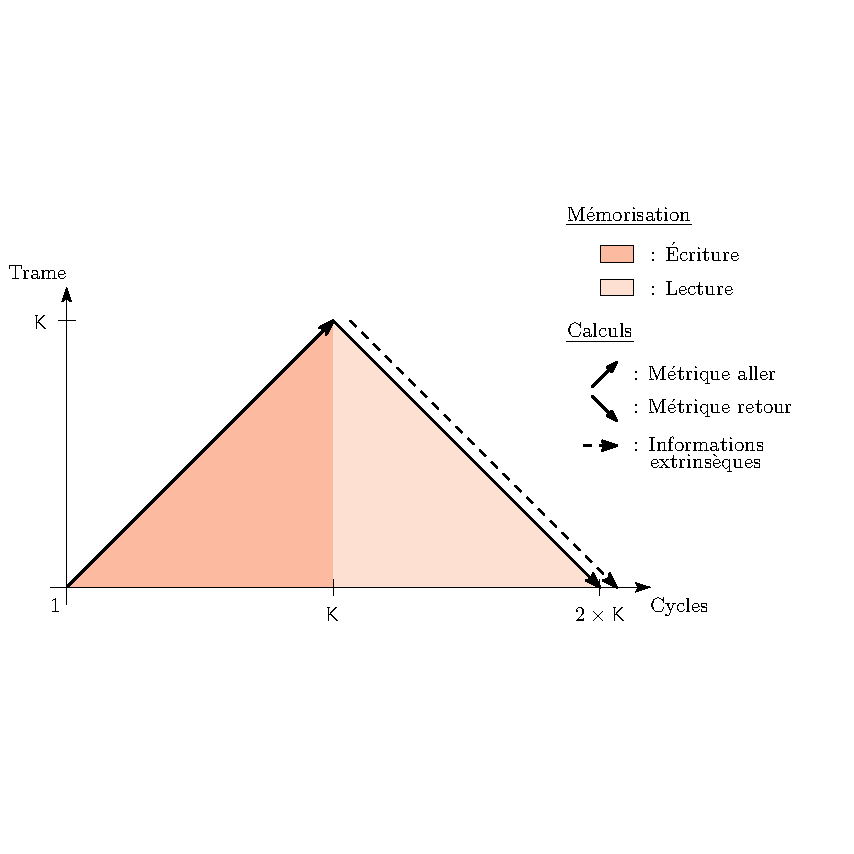
\includegraphics{main/ch4_fig/ipe/FB+LEG.pdf}
	\caption{BCJR Aller-Retour (FB). \label{fig:siso_seq}}
\end{figure}

\paragraph*{BCJR aller-retour avec fenêtre glissante}
À partir cette ordonnancement, la technique de fenêtre glissante (sliding-window) a été proposée. Son objectif réside e
n la réduction de la mémorisation nécessaire. Son principe est le suivant. La trame à décoder est découpée en W fenêtres 
de tailles égales. Après avoir calculé K/W métriques de nœuds aller, le calcul de la métrique de nœuds retour débute 
en commençant à l'index de la trame K/W. Vient ensuite celui des informations \textit{a posteriori}. À la fin de la 
récursion retour, une autre fenêtre de la trame est considérée. Ceci est répété jusqu'à ce que l'ensemble de la trame
soit traitée. Les besoins de mémorisations passent ainsi à K/W métriques de nœud. Cependant, la suppression de la 
récursion aux limites des sous trames implique une dégradation  des performances de décodages. Pour palier à cela, deux 
techniques sont possibles. Il s'agit de l'utilisation : 
\begin{itemize}
	\item d'une fenêtre d'acquisition. Dans ce cas, le calcul des métriques de nœud retour est commencé sur 
	quelques sections de treillis suivant la limite de la taille du sous bloc. Une étude empirique a montré que la 
	taille de ce prologue présentant le meilleur compromis entre calcul supplémentaires et amélioration des performances de décodage est situé entre 3 et 5 fois la longueur de contrainte du code \cite{sw_init}.
	\item du passage de messages. Son principe consiste à utiliser les métriques de nœud calculées lors de l'itération précédente en tant que valeurs initiales à la limite de chaque bloc. Cette technique propose de meilleurs performances de décodage que la technique de la fenêtre d'acquisition pour un surcoût de mémorisation limité.
\end{itemize}
Si, l'ordre des calculs est inversé, c'est à dire si en premier lieu le calcul des métriques de nœud retour est 
effectué, il est possible de produire les informations extrinsèques dans l'ordre en n'utilisant plus que $K/W + K$
cycles. Dans ce cas, les unités de calcul de nœuds aller et retour se doivent de fonctionner en même temps. Ceci ne 
nécessite pas de ressources matérielle supplémentaires puisqu'elles sont déjà présentes dans le cas de l'ordonnancement 
FB. Les besoins en mémorisation sont en revanche réduits à $K/W$. Cet ordonnancement est nommé dans la suite 
Backward-Forward-Sliding-Window (BF-SW). La Figure \ref{fig:siso_sw} schématise un tel ordonnancement pour $W=2$.

\begin{figure}[!h]
	\centering
	\includegraphics{main/ch4_fig/ipe/BF_SW.pdf}
	\caption{BCJR Retour-Aller avec fenêtre glissante (BF-SW). \label{fig:siso_sw}}
\end{figure}

\subsubsection{BCJR parallèle}
\paragraph*{BCJR en aile de papillon}
À partir de l'ordonnancement BF-SW, en ne considérant qu'une seule fenêtre mais en doublant de le nombre d'unités de 
calcul d'information \textit{a posteriori}, il est possible de débuter les calculs récursifs des métriques de nœuds 
aller et des métriques de nœuds retour en même temps. Dans ce cas, à partir de a moitié du parcours du treillis, deux 
informations extrinsèques sont produites en même temps. Cet ordonnancement est nommé BCJR en aile de papillon (Butterfly, abrégé en BFLY dans 
la suite) \cite{butterfly} et est est présenté en Figure \ref{fig:siso_but}. De la sorte, uniquement $K$ cycles 
d'horloge sont nécessaires pour effectuer une demi-itération de turbo décodage. L'effort de mémorisation reste inchangé 
par rapport au BCJR aller-retour. En revanche les informations extrinsèques sont produites par paires à partir du $K/2^{\text{ième}}$ cycle. Cette ordonnancement permet donc de réduire la latence du turbo décodage d'un facteur deux vis-à-vis de l'ordonnancement FB.

% \begin{figure}[h]
% 	\centering
% 	\includegraphics{main/ch4_fig/ipe/BFLY.pdf}
% 	\caption{BCJR Butterfly (BFLY). \label{fig:siso_but}}
% \end{figure}

\paragraph*{BCJR en aile de papillon et fenêtre glissante}
Toujours dans un but de réduction des éléments de mémorisation, il est possible d'utiliser le concept de fenêtre 
glissante sur l'ordonnancement BFLY. Comme à partir de l'ordonnancement FB, le découpage de la trame en W fenêtres permet de réduire les ressources de mémorisation par un facteur W. Cependant, dans ce cas, aucun gin en latence ne peut
être obtenu. La Figure \ref{fig:siso_bf_sw} présente cet ordonnancement (abrégé en BFLY-SW) pour $W = 2$. Dans ce cas, 
les informations extrinsèques sont produites en deux salves de 2 informations extrinsèques de durée K/4.

% \begin{figure}[!h]
% 	\centering
% 	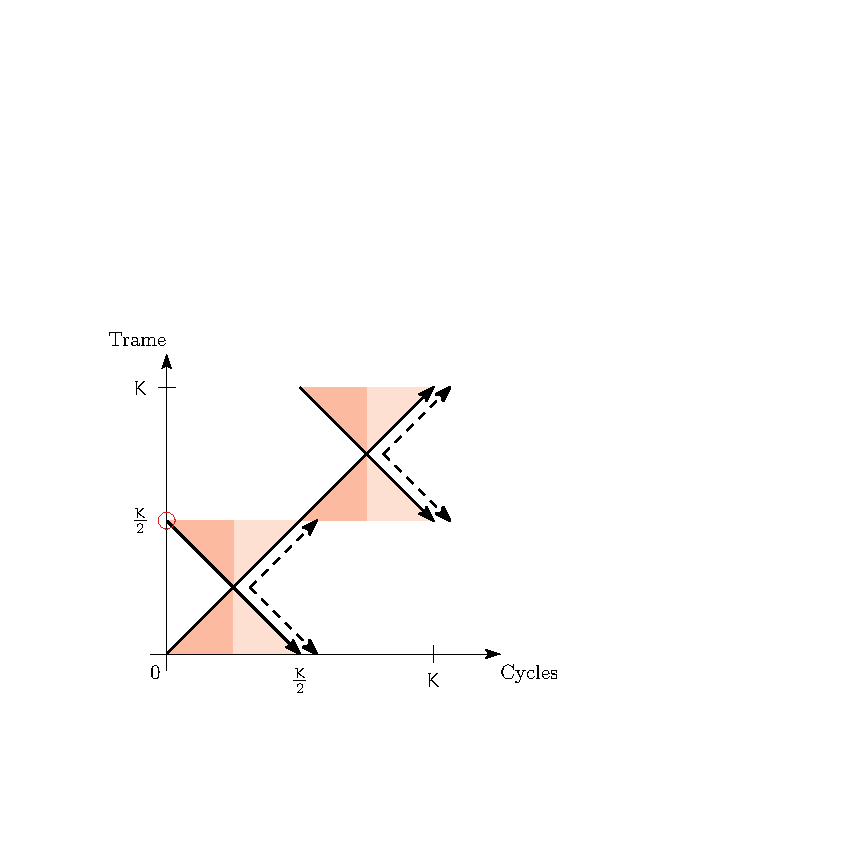
\includegraphics{main/ch4_fig/ipe/BFLY_SW.pdf}
% 	\caption{BCJR Butterfly avec fenêtre glissante (BFLY-SW). \label{fig:siso_bf_sw}}
% \end{figure}

\begin{figure}[!h]
    \centering
    \begin{minipage}[t]{.49\textwidth}
	\centering
	\includegraphics{main/ch4_fig/ipe/BFLY.pdf}
	\caption{BCJR Butterfly (BFLY). \label{fig:siso_but}}
    \end{minipage}~~~~~~%
    \begin{minipage}[t]{0.49\textwidth}
	\centering
	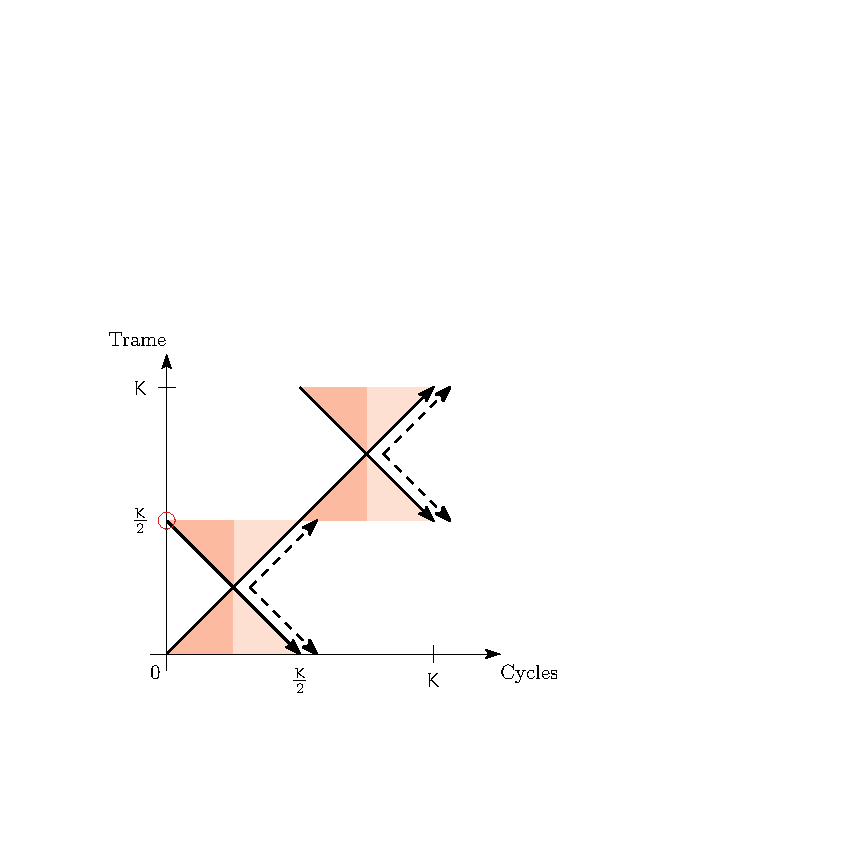
\includegraphics{main/ch4_fig/ipe/BFLY_SW.pdf}
	\caption{BCJR Butterfly avec fenêtre glissante (BFLY-SW). \label{fig:siso_bf_sw}}
    \end{minipage}
\end{figure}

\subsection{Processus itératif parallèle}
Il est possible d'agir sur d'autres niveaux de parallélisme en plus de celui du BCJR. Tout d'abord un 
parallélisme opérant au niveau du calcul d'une demi itération est présente.
\subsubsection{Parallélisme à l'intérieur d'une demi-itération}
À partir de l'algorithme par fenêtre glissante, afin de gagner un niveau de parallélisme supplémentaire, il est possible 
d'augmenter le nombre de décodeurs SISO fonctionnant en même temps. Chacun opère alors sur une fenêtre différente de la 
trame. La Figure \ref{fig:turbo_par} illustre un tel degré de parallélisme pour un nombre de sous blocs de deux ($B=2$).
Dans ce cas, deux décodeurs SISO se répartissent sur la trame, l'un s'occupant des informations allant de l'index
1 à K/2, l'autre de K/2+1 à K. À nouveau, une initialisation aux limites des sous-trames est nécessaire. Les mêmes 
techniques que présentées précédemment peuvent être envisagées. Cependant, cette fois, en plus des métrique de nœuds
retour, les métriques de nœud aller doivent aussi être considérées. Aussi ce degré de parallélisme nécessite que 
l'entrelaceur puisse lui aussi être parallélisé afin qu’aucun conflit d'accès ne puisse apparaître 
\cite{interleaver_conflict}. 
La temps nécessaire pour effectuer une demi itération est alors réduit d'un facteur $B$. Cependant, les ressources 
matérielles sont multipliées par ce même facteur.

\begin{figure}[!h]
	\centering
	\includegraphics{main/ch4_fig/ipe/parallel.pdf}
	\caption{Turbo décodage parallèle. \label{fig:turbo_par}}
\end{figure} 

Le choix de l'ordonnancement pour chaque décodeur SISO est libre. La Figure \ref{fig:sisos_par} présente un niveau de 
parallélisme de 2 à partir de l'ordonnancement BFLY pour un nombre de sous-blocs valant 2. Cet ordonnancement est nommé BFLY-SB dans la suite. Il apparaît que dans ce cas, K/2 cycles sont nécessaires pour effectuer une demi itération. 
Durant les K/4 derniers cycles, 4 informations extrinsèques sont produites en parallèle. Finalement, le nombre de
ressources de mémorisation vaut K métriques de nœuds.

Afin de réduire les besoins de mémorisation, il est possible de combiner le parallélisme de sous-bloc avec le principe 
de fenêtre glissante. De la sorte, en considérant W fenêtres différentes, la taille de la mémoire est réduite d'un 
facteur W au niveau des métriques de nœud. La Figure \ref{fig:sisos_par_sb} présente un ordonnancement Butterfly avec 
2 fenêtres de glissement et un parallélisme de sous-bloc de 2. Cet ordonnancement est nommé BFLY-SB-SW dans la suite.

\begin{figure}[!h]
    \centering
    \begin{minipage}[t]{.49\textwidth}
        \centering
        \includegraphics{main/ch4_fig/ipe/BFLY_SB.pdf}
		\caption{SISO Butterfly en parallèle (BFLY-SB). \label{fig:sisos_par}}
    \end{minipage}~~~~~~%
    \begin{minipage}[t]{0.49\textwidth}
        \centering
        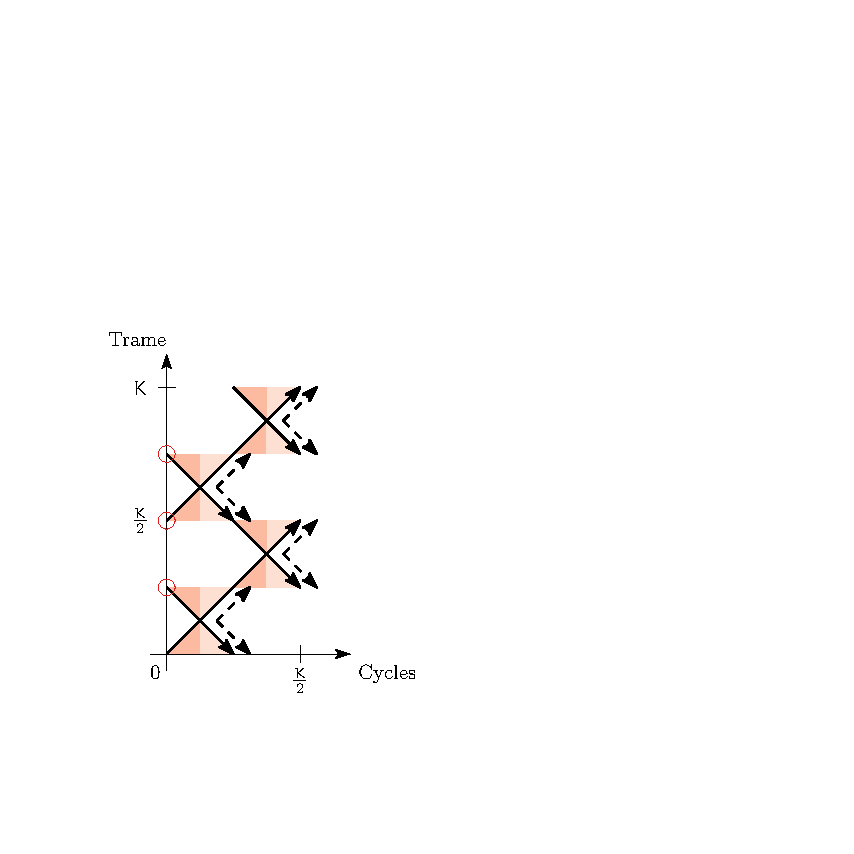
\includegraphics{main/ch4_fig/ipe/BFLY_SB_SW.pdf}
		\caption{SISO Butterfly avec fenêtre glissante en parallèle (BFLY-SW-SB). \label{fig:sisos_par_sb}}
    \end{minipage}
\end{figure}

\subsubsection{Parallélisme entre les itérations}
Plus encore, il est possible de considérer un autre niveau de parallélisme. Il est en effet possible de faire opérer le 
décodage de deux codes composant le turbo décodeur en même temps \cite{turbo_par}. Dans ce cas, après chaque itération, 
chaque décodeur élémentaire travaillant dans un certain domaine fourni ses informations extrinsèques au décodeur 
élémentaire utilisant les données du canal de l'autre dimension. Cependant, cette technique nécessite à performances de 
décodage égales deux fois plus d'itérations que le turbo décodage conventionnel. Ceci vient du fait que le principe itératif du turbo décodage conventionnel n'est plus respectée dans ce cas.

Pour palier à cela, en 2005, le décodage shuffled a été proposé \cite{turbo_shuff}. Le principe est similaire à celui 
présenté à l'instant. Cependant, les informations extrinsèques sont échangées entre les deux domaines dès qu'elles ont 
été calculées. Chaque décodeur composant a donc accès plus vite aux information \textit{a priori} mises à jour. Ceci a 
alors pour effet d'augmenter la vitesse de convergence et permet donc d'approcher les mêmes besoin en itération qu'avec
un turbe décodage conventionnel pour des performances de décodage équivalentes. Il est cependant à noter que ceci est 
vrai en considérant un ordonnancement Butterfly-Replica \cite{butt_replica}. Celui-ci permet, au prix d'un doublement de 
la mémoire de métriques de nœud, de produire des informations extrinsèques durant toute la durée de la durée itération, 
participant à l'augmentation de la vitesse de convergence.
La Figure \ref{fig:turbo_shuff} présente un échange d'informations extrinsèques au cours du processus de décodage shuffled avec deux décodeurs composants travaillant en simultané.

Pour de telles implémentations de turbo décodeurs, une vision utilisant de multiples processeurs à jeu d’instruction à application spécifique (ASIP) sera préférée \cite{asip}.

\begin{figure}[!h]
	\centering
	\includegraphics{main/ch4_fig/ipe/shuffled.pdf}
	\caption{Turbo décodage Shuffled. \label{fig:turbo_suff}}
\end{figure}

Enfin la dernière méthode permettant de paralléliser le processus itératif de décodage revient à dupliquer l'ensemble 
du turbo décodeur afin de décoder différentes trames en même temps. Cette méthode revient à utiliser une architecture 
pipeline pour le décodeur. Dans ce cas, la profondeur maximale du pipeline équivaut à deux fois le nombre d'itération 
maximal permis. Bien que permettant une augmentation 
conséquente du débit, cette approche ne réduit pas la latence du processus de décodage alors qu'elle est coûteuse sur 
le plan matériel puisque toutes les ressources calculatoires et de mémorisation sont dupliquées.

\subsection{Conclusions}
\begin{table}[b]
\centering
\caption{TITRE}
\label{tab:compa}
\resizebox{\textwidth}{!}{
\begin{tabular}{rllll}
\toprule
Ordonnancement      & Durée Demi-Iter   & Durée Itération   & Durée transmission ext   & Nb ext en //   \\
\cmidrule(r){1-1}      \cmidrule(l){2-2}      \cmidrule(l){3-3}      \cmidrule(l){4-4}             \cmidrule(l){5-5}    
FB 		            & 2K                & 4k                & K                        & 1              \\
BF-SW (W)           & K + K/W           & 2(K + K/W)        & K                        & 1              \\
BFLY                & K                 & 2K                & K/2                      & 2              \\
BFLY-SW (W)         & K                 & 2K                & K/2 = W(K/(2W))          & 2              \\
BFLY-PAR (Q)        & K/Q               & 2(K/Q)            & K/(2Q)                   & 2Q             \\
BFLY-SW-PAR (W,Q)   & K/Q               & 2(K/Q)            & K/(2Q) = W(K/(2QW))      & 2Q             \\
\bottomrule
\end{tabular}}
\end{table}


%%%%%%%%%%%%%%%%%%%%%%%%%%%%%%%%%%%%%%%%%%%%%%%%%%%%%%%%%%%%%%%%%%%%%%%%%%%%%%%%%%%%%%%%%%%%%%%%%%%%%%%%%%%%%%%%%%%%%%%%
\newpage
\section{Études de l'impact des paramètres de l'algorithme FNC}
L'algorithme FNC est fonction de plusieurs paramètres ayant un impact à la fois sur les performances de décodage et sur
la complexité calculatoire. Cette section vise à étudier l'impact de chacun de ces paramètres sur les performances de 
décodage dans le cadre de turbo codes du standard LTE. Pour ce faire, une variation indépendante de chacun de ces 
paramètres est mené.

Vis-à-vis de l'algorithme \ref{alg:fc_b} présenté dans le chapitre précédent, une première modification est effectuée. 
Dorénavant, l'application de l'algorithme FNC n'est plus réalisé après la demi-itération dans le domaine
entrelacé mais après la demi-itération dans le domaine naturel. De la sorte, il n'est plus nécessaire d'effectuer une 
opération de désentrelacement avant de pouvoir effectuer l'algorithme FNC.

\subsection{Paramètres liés aux itérations}
Le premier groupe de paramètres correspond au choix des itérations du processus de turbo décodage sur lesquelles le 
principe FNC est appliqué. Il a été introduit dans le chapitre précédent que si l'itération minimale à partir de 
laquelle l'algorithme est trop faible, alors les performances de décodages peuvent être dégradées. Ceci dépend du risque 
d'erreur non détectée par le code détecteur d'erreurs. Cette probabilité est fonction de la taille de trame et de la 
taille du code CRC. En effet, pour une taille du code CRC constante, la probabilité d'erreur non détectée croît avec la
taille de la trame. 

La Figure \ref{fig:fnc_minX} présente l'impact sur les performances de décodage de l'algorithme FNC avec $q=10$ de la 
valeur de l'itération à partir de laquelle l'algorithme commence à être appliqué (paramètre $I_\text{min}$), ce pour 
différents turbo codes du standard LTE. Dans ces trois cas, $I_\text{min}$ évolue de 2 à 8. L'algorithme est donc 
appliqué respectivement de 7 à 1 fois. Il apparaît alors que pour chacun de ces codes, il existe une valeur optimale de 
$I_\text{min}$, faisant apparaître les meilleures performances de décodage. Elle s'établit à 3 pour K=528 et à 5 pour 
K=2048 ou 6144. Cette valeur optimale est notée $I_{\text{m}_\text{o}}$. En deçà de cette valeur, la trop forte occurrence 
d'erreurs non détectées lors de la vérification du 
code CRC dégrade les performances de décodage. Au delà de cette valeur $I_\text{min}$, à chaque fois qu'elle est 
incrémentée, les performances de décodage s'amenuisent légèrement.

\begin{figure}[!h]
	\centering 
	\hspace*{-.075\textwidth}
	\includegraphics[width=1.1\textwidth]{main/ch4_fig/final/tikz_last/fnc10_minX.pdf}
	\caption{Comparaison des performances de décodage de l'algorithme FNC pour $q=10$ et différentes valeurs de 
	$I_\text{min}$. Turbo codes du standard LTE de rendement 1/3. 
	Turbo décodeur basé sur l'algorithme EML-MAP itérant au plus 8 fois.
	\label{fig:fnc_minX}}
\end{figure}

Afin de dresser l'impact de chacune des itérations à laquelle l’algorithme FNC est appliqué, la Figure 
\ref{fig:fnc_onlyX} présente les performances de décodage avec une seule application de l'algorithme FNC pour le 
turbo code K=2048 (noté $@i=n$). Les valeurs de $i$ présentant de moins bonnes performances de décodages que celles 
obtenues avec l'algorithme de décodage conventionnel sont exclues. Ceci est alors opposé aux performances de décodage 
obtenues avec $I_\text{min} = I_{\text{m}_\text{o}}$. Il apparaît alors que n'appliquer qu'une seule l'approche FNC par 
trame dégrade les performances de décodage en comparaison avec l’application à chaque itération à partir de $I_\text{min}
 = I_{\text{m}_\text{o}}$. Cependant cette dégradation est minime puisqu'elle ne représente qu'un facteur deux dans le 
 pire des cas.

\begin{figure}[!h]
	\centering 
	\hspace*{-.075\textwidth}
	\includegraphics[width=1.1\textwidth]{main/ch4_fig/final/tikz_last/fnc10_onlyX.pdf}
	\caption{Comparaison des performances de décodage de l'algorithme FNC pour $q=10$ et appliqué à une seule itération. 
	Turbo codes du standard LTE de rendement 1/3. 
	Turbo décodeur basé sur l'algorithme EML-MAP itérant au plus 8 fois.
	\label{fig:fnc_onlyX}}
\end{figure}

Finalement, il peut être intéressant de ne considérer l'application de l'algorithme uniquement toutes les deux 
itérations. Ceci permettrait alors d'obtenir une budget temps plus conséquent pour effectuer l'algorithme FNC. Le Figure 
\ref{fig:fnc_step} présente alors la différence de performance pour ces mêmes turbo codes du standard LTE dans les cas
où $I_\text{min} = I_{\text{m}_\text{o}}$ mais en considérant une application du principe FNC soit toute les itérations 
soit toutes les deux itérations (noté Pas=2). Dans ce dernier cas, pour K=528, 3 applications du principe FNC sont 
considérées. Pour K=2048 et K=6144, ce sont 2 applications qui sont considérées. Leur nombre est donc divisé par 2 dans 
chaque cas vis-à-vis de la référence. Dans ce cas, la dégradation des performances est très légère et donc moins 
importante que dans le cas précédent.

\begin{figure}[!h]
	\centering
	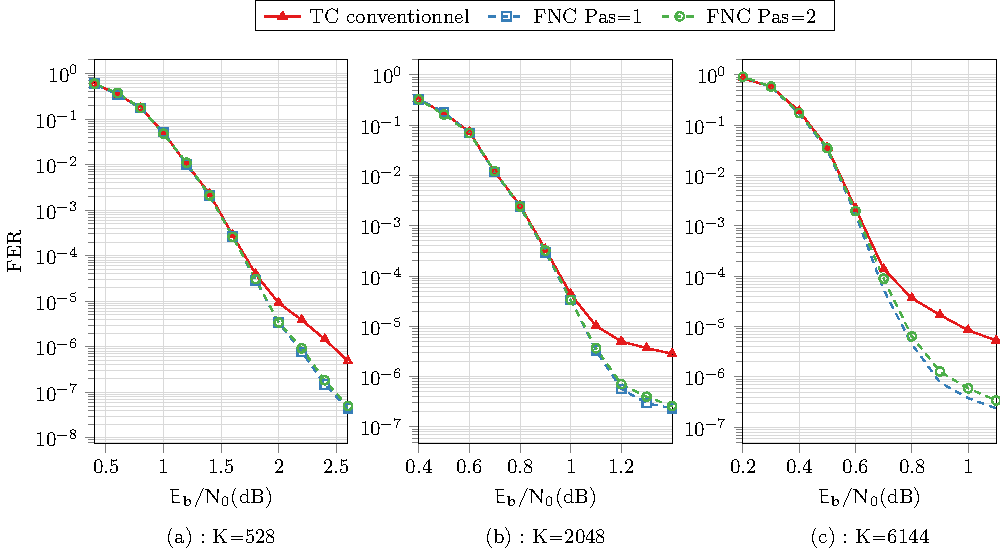
\includegraphics[width=.9\textwidth]{main/ch4_fig/final/tikz_last/fnc10_minO_s2.pdf}
	\caption{Performances de l'algorithme FNC appliqué toutes les deux itérations ($I_\text{FNC}$) pour différentes 
	valeurs de K, $q=10$.
	Turbo décodeur basé sur l'algorithme EML-MAP itérant au plus 8 fois.
	\label{fig:fnc_step}}
\end{figure}

En conclusion de cette étude, une trop faible valeur de $I_\text{min}$ est néfaste aux performances de l'algorithme. 
La valeur optimale de $I_\text{min}$ en terme de performances de décodages résultantes est entièrement dépendante des
capacités de détection du code détecteur d'erreur. L'application de l'algorithme FNC après chaque itération de turbo 
décodage permet d'obtenir les meilleures performances de décodage. Chaque suppression d'application du principe FNC 
dégrade les performances optimales. Néanmoins, ne pas appliquer à chaque itération l'algorithme mais toutes les deux 
itérations permet d'augmenter le budget temps pour le traitement de cet algorithme tout en n'impactant que très légèrement 
les performances de décodage. Ceci permettra donc de réduire la complexité matérielle de 
l'implémentation de l'algorithme FNC et sera détaillé dans une section prochaine de ce chapitre.

Maintenant, l'étude de l'impact de la valeur de $q$, correspondant à la profondeur de recherche, est mené.

\subsection{Impact de la taille de recherche}
Il a été présenté dans le chapitre précédent que les performances de l'algorithme FNC était très fortement conditionnées
par la taille du vecteur de recherche de positions probablement erronées $q$. En effet, incrémenter $q$ de $1$ revient 
à considérer deux fois plus de mots candidats. Ceci augmente de fait la probabilité d'identifier le bon mot de code. 
Cependant, la complexité calculatoire se voit donc doublée pour chaque incrément de $q$. 

\begin{figure}[!t]
	\hspace*{-.075\textwidth}
	\includegraphics[width=1.1\textwidth]{main/ch4_fig/final/tikz_last/fnc_qX.pdf}
	\caption{Performances de l'algorithme FNC appliqué toutes les deux itérations ($I_\text{FNC}$) pour différentes 
	valeurs de K, et de $q$.
	Turbo décodeur basé sur l'algorithme EML-MAP itérant au plus 8 fois.
	\label{fig:fnc_q}}
\end{figure}

La Figure \ref{fig:fnc_q} présente l'impact de l'évolution de la valeur de $q$ pour les turbo codes du standard LTE 
d'une taille de trame allant de K=528 à K=6144. Dans tous les cas, l'algorithme FNC est utilisé toutes les itérations à 
partir de l'itération $I_\text{min} = I_{\text{m}_\text{o}}$ telles que les performances de décodages 
soient les meilleures pour $q=10$. Dans l'ensemble, comme attendu, il apparaît que la réduction de $q$ impacte 
négativement les performances de décodage. Cependant, cet impact dépend du turbo ode considéré. Par exemple, pour 
$K=528$, le passage de $q=10$ à $q=8$ a un impact plus défavorable que le passage de $q=8$ à $q=6$. Ceci s'explique par
la distribution des erreurs binaires de ce turbo code. En effet, une part non négligeable des trames erronées contiennent
9 erreurs (cf. Figure \ref{fig:be}). Elles ne peuvent donc être corrigées seulement dans les cas tels que $q\geq 9$. En 
revanche, pour $K=2048$, la très grande majorité des trames erronées contiennent strictement moins de 6 erreurs binaires.
Ceci explique la similitude des performances de décodage pour une valeur de $q$ comprise entre 10 et 6. Cependant, le 
passage de q=6 à q=4 impacte plus négativement les performances de décodage de l'algorithme FNC.

Finalement il apparaît que la valeur de $q$ proposant le meilleur ratio entre amélioration des performances de décodage 
dépend fortement du turbo code considéré. Plus la valeur de $q$ est grande, meilleures sont les performances. Cependant,
passé, $q=9$, dans les trois cas considérés n'apportent que des gains marginaux. Ceci serait à nuancer dans le contexte 
d'un autre standard considérant un code CRC possédant de meilleures propriétés de distance.

Le dernier vecteur de modifications de l'algorithme FNC pour son implémentation concerne la représentation de 
l'information en virgule fixe. Ceci est l'objet de la prochaine section.

\subsection{L'algorithme FNC et la quantification de l'information}
Dans un premier temps, il est nécessaire de vérifier que l'algorithme FNC supporte un passage en virgule fixe. Pour ce 
faire, les performances de décodages sont comparées suivant le format des données internes aux turbo décodeurs. Les 
formats considérés sont soit une représentation flottante de l'information, soit une quantification des données internes 
sur 16 bits, soit enfin, une quantification sur 8 bits. Les performances de décodage en activant ou non le principe FNC 
sont présentées en Figure \ref{fig:fnc_format_refs}. Il apparaît alors que le passage en représentation à virgule fixe 
induit une dégradation des performances de décodage du turbo décodeur conventionnel en regard des celles obtenues avec 
une représentation flottante. Cette dégradation est très légère dans le cas d'une limitation à 16 bits. Elle est un peu 
plus marquée dans le cas où les données sont sur 8 bits. \textcolor{blue}{Cette même dégradation apparaît lors de 
l'emploi du principe FNC avec une représentation des données en virgule fixe. Ainsi, les gains en performance de 
décodage sont conservés malgré le changement de représentation de l'information.}

\begin{figure}[!h]
	\centering
	\includegraphics[width=.9\textwidth]{main/ch4_fig/final/tikz_last/fnc10_format_refs.pdf}
	\caption{Comparaison des performances de l'algorithme FNC $q=10$ pour différents turbo codes du standard LTE, 
	suivant la représentation de l'information choisie.
	Turbo décodeur basé sur l'algorithme EML-MAP itérant au plus 8 fois.
	\label{fig:fnc_format_refs}}
\end{figure}

Comme la métrique $\Delta$ de l'algorithme FNC est basée sur la valeur absolue d'une somme, sa dynamique reste identique 
à celle des opérandes. Or, comme la métrique $\Delta$  est utilisée en ses positions minimales, il est possible de 
saturer la dynamique des données sans impacter les performances d'identification. Ceci est démontré en Figure 
\ref{fig:fnc_format_8b}. Dans ce cas, le turbo décodeur manipule des données sur 8 bits. Le nombre de bits utilisés pour 
la métrique $\Delta$, noté $b_{\Delta}$ varie alors de 8 à 4. Il apparaît alors que lorsque $b_{\Delta}$ vaut 8, 7 ou 6,
les performances de décodage sont strictement identiques. A partir de $b_{\Delta} = 5$ une légère dégradation des 
performances de décodage apparaît. Cette dernière augmente fortement pour $b_{\Delta} = 4$. Dans ce cas, la dynamique 
de la métrique $\Delta$ n'est plus suffisante pour réussir à ordonner correctement les positions problématiques.

\begin{figure}[!t]
	\hspace*{-.075\textwidth}
	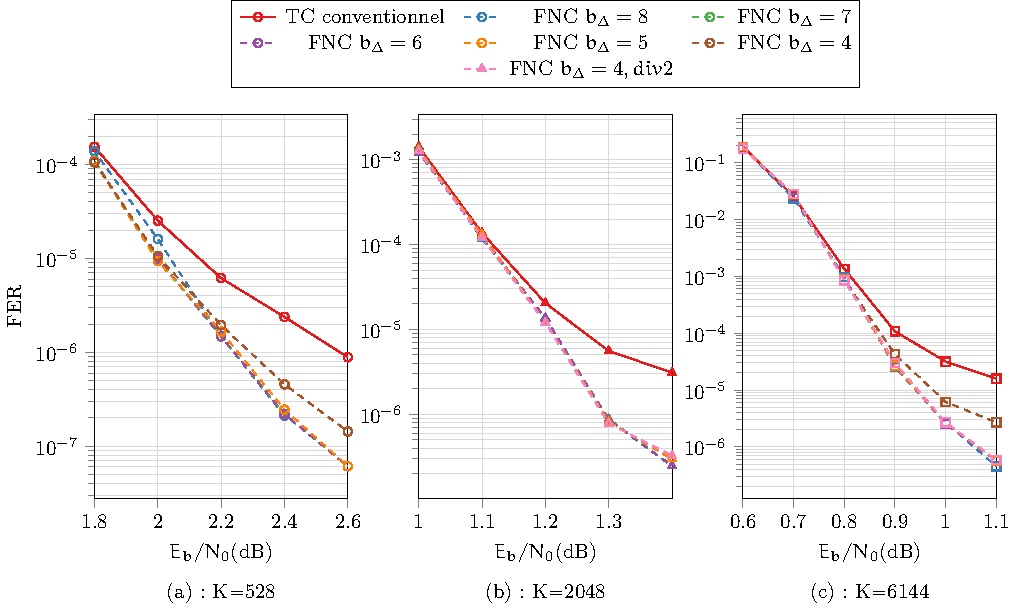
\includegraphics[width=1.1\textwidth]{main/ch4_fig/final/tikz_last/fnc10_format_8b.pdf}
	\caption{Performances de l'algorithme FNC pour différents turbo codes du standard LTE, selon la dynamique $b_{\Delta}$ 
	de la métrique $\Delta$.
	Turbo décodeur 8 bits basé sur l'algorithme EML-MAP itérant au plus 8 fois.
	\label{fig:fnc_format_8b}}
\end{figure}

En conclusion, pour un turbo décodeur utilisant 8 bits pour ses métriques internes, \textcolor{blue}{fixer la valeur de $b_{\Delta}$ 
à 6} permet de limiter la dynamique des données en entrée de l'algorithme FNC tout en fournissant 
rigoureusement les mêmes performances de décodage que celles obtenues sans saturation.

\subsection{Conclusion}
Dans cette section, une étude de l'impact des différents paramètres de l'algorithme FNC a été menée. Ces paramètres ont
pour la plupart un impact sur les performances de décodage et la complexité calculatoire de l'algorithme FNC. Suivant 
les performances de décodage visées et l'ajout de complexité calculatoire toléré, le concepteur d'un turbo décodeur 
utilisant l'algorithme FNC devra choisir les valeurs de ces différents paramètres en conséquence.

La section suivante présente une architecture matérielle pour l'algorithme FNC dans le contexte d'un turbo décodeur 
séquentiel basé sur l'ordonnancement Backward-Forward-Sliding-Window. L'impact sur la complexité matérielle des 
paramètres précédents sera alors étudiée.